\documentclass{beamer}

%
% Common preamble for all three parts.
%
\usepackage[spanish]{babel}
\usepackage{amsmath}
\usepackage{color}
\ProvidesPackage{minted}
\usepackage{minted}
%\setminted{encoding=utf8}
\usepackage{hyperref}
\usepackage{multicol}
\usepackage{tabularx}
\usepackage{tikz}

\usepackage[utf8]{inputenc}
%\usepackage{ucs}
%\usepackage[T1]{fontenc}
%\newcommand{\minted@encoding}{\minted@get@opt{encoding}{UTF8}}

% only inline todonotes work
\usepackage{xkeyval}
\usepackage[textsize=small]{todonotes}
\presetkeys{todonotes}{inline}{}

\usetikzlibrary{shapes,arrows,positioning,shadows}

% no nav buttons
\usenavigationsymbolstemplate{}

\newcommand{\bftt}[1]{\textbf{\texttt{#1}}}
\newcommand{\comment}[1]{{\color[HTML]{008080}\textit{\textbf{\texttt{#1}}}}}
\newcommand{\cmd}[1]{{\color[HTML]{008000}\bftt{#1}}}
\newcommand{\bs}{\char`\\}
\newcommand{\cmdbs}[1]{\cmd{\bs#1}}
\newcommand{\lcb}{\char '173}
\newcommand{\rcb}{\char '175}
\newcommand{\cmdbegin}[1]{\cmdbs{begin\lcb}\bftt{#1}\cmd{\rcb}}
\newcommand{\cmdend}[1]{\cmdbs{end\lcb}\bftt{#1}\cmd{\rcb}}

\newcommand{\wllogo}{\textbf{Overleaf}}

% this is where the example source files are loaded from
% do not include a trailing slash
\newcommand{\fileuri}{https://raw.github.com/guanucoluis/latex-course/master/es}

\newcommand{\wlserver}{https://www.overleaf.com}
\newcommand{\wlnewdoc}[1]{\wlserver/docs?snip\_uri=\fileuri/#1\&splash=none}

\def\tikzname{Ti\emph{k}Z}

% from http://tex.stackexchange.com/questions/5226/keyboard-font-for-latex
\newcommand*\keystroke[1]{%
  \tikz[baseline=(key.base)]
    \node[%
      draw,
      fill=white,
      drop shadow={shadow xshift=0.25ex,shadow yshift=-0.25ex,fill=black,opacity=0.75},
      rectangle,
      rounded corners=2pt,
      inner sep=1pt,
      line width=0.5pt,
      font=\scriptsize\sffamily
    ](key) {#1\strut}
  ;
}
\newcommand{\keystrokebftt}[1]{\keystroke{\bftt{#1}}}

% stolen from minted.dtx
\newenvironment{exampletwoup}
  {\VerbatimEnvironment
   \begin{VerbatimOut}{example.out}}
  {\end{VerbatimOut}
   \setlength{\parindent}{0pt}
   \fbox{\begin{tabular}{l|l}
   \begin{minipage}{0.55\linewidth}
     \inputminted[fontsize=\small,resetmargins]{latex}{example.out}
   \end{minipage} &
   \begin{minipage}{0.35\linewidth}
     \input{example.out}
   \end{minipage}
   \end{tabular}}}

\newenvironment{exampletwouptiny}
  {\VerbatimEnvironment
   \begin{VerbatimOut}{example.out}}
  {\end{VerbatimOut}
   \setlength{\parindent}{0pt}
   \fbox{\begin{tabular}{l|l}
   \begin{minipage}{0.55\linewidth}
     \inputminted[fontsize=\scriptsize,resetmargins]{latex}{example.out}
   \end{minipage} &
   \begin{minipage}{0.35\linewidth}
     \setlength{\parskip}{6pt plus 1pt minus 1pt}%
     \raggedright\scriptsize\input{example.out}
   \end{minipage}
   \end{tabular}}}

\newenvironment{exampletwouptinynoframe}
  {\VerbatimEnvironment
   \begin{VerbatimOut}{example.out}}
  {\end{VerbatimOut}
   \setlength{\parindent}{0pt}
   \begin{tabular}{l|l}
   \begin{minipage}{0.55\linewidth}
     \inputminted[fontsize=\scriptsize,resetmargins]{latex}{example.out}
   \end{minipage} &
   \begin{minipage}{0.35\linewidth}
     \setlength{\parskip}{6pt plus 1pt minus 1pt}%
     \raggedright\scriptsize\input{example.out}
   \end{minipage}
   \end{tabular}}

\title{Una Introducción Interactiva a \LaTeX}
\author{Siria Sadeddin}


\subtitle{Parte 3: No Solo Documentos de Texto: Presentaciones y Más}

\newcommand{\alicia}[1]{\todo[color=green!40]{#1}}
\newcommand{\juan}[1]{\todo[color=purple!40]{#1}}

\begin{document}

%%%%%%%%%%%%%%%%%%%%%%%%%%%%%%%%%%%%%%%%%%%%%%%%%%%%%%%%%%%%%%%%%%%%%%%%%%%%%%%
%%%%%%%%%%%%%%%%%%%%%%%%%%%%%%%%%%%%%%%%%%%%%%%%%%%%%%%%%%%%%%%%%%%%%%%%%%%%%%%
%%%%%%%%%%%%%%%%%%%%%%%%%%%%%%%%%%%%%%%%%%%%%%%%%%%%%%%%%%%%%%%%%%%%%%%%%%%%%%%
\begin{frame}
  \titlepage
\end{frame}


%%%%%%%%%%%%%%%%%%%%%%%%%%%%%%%%%%%%%%%%%%%%%%%%%%%%%%%%%%%%%%%%%%%%%%%%%%%%%%% 
%%%%%%%%%%%%%%%%%%%%%%%%%%%%%%%%%%%%%%%%%%%%%%%%%%%%%%%%%%%%%%%%%%%%%%%%%%%%%%%
%%%%%%%%%%%%%%%%%%%%%%%%%%%%%%%%%%%%%%%%%%%%%%%%%%%%%%%%%%%%%%%%%%%%%%%%%%%%%%%
\section{Presentaciones con  \protect\bftt{beamer}}

%%%%%%%%%%%%%%%%%%%%%%%%%%%%%%%%%%%%%%%%%%%%%%%%%%%%%%%%%%%%%%%%%%%%%%%%%%%%%%% 
%%%%%%%%%%%%%%%%%%%%%%%%%%%%%%%%%%%%%%%%%%%%%%%%%%%%%%%%%%%%%%%%%%%%%%%%%%%%%%% 
%%%%%%%%%%%%%%%%%%%%%%%%%%%%%%%%%%%%%%%%%%%%%%%%%%%%%%%%%%%%%%%%%%%%%%%%%%%%%%% 
\begin{frame}[fragile]{\insertsection}
  \begin{itemize}
  \item Beamer es un paquete para crear presentaciones  en \LaTeX{}.
  \item Se dispone de una clase de documentos  \bftt{beamer}.
  \item Utilice el entorno  \bftt{frame} para crear diapositivas (cuadros).
  \end{itemize}
  \begin{minipage}{0.55\linewidth}
    \inputminted[fontsize=\scriptsize,frame=single,resetmargins]{latex}%
    {es/beamer-minimal.tex}
  \end{minipage}
  \begin{minipage}{0.35\linewidth}
    % trim: l b r t
    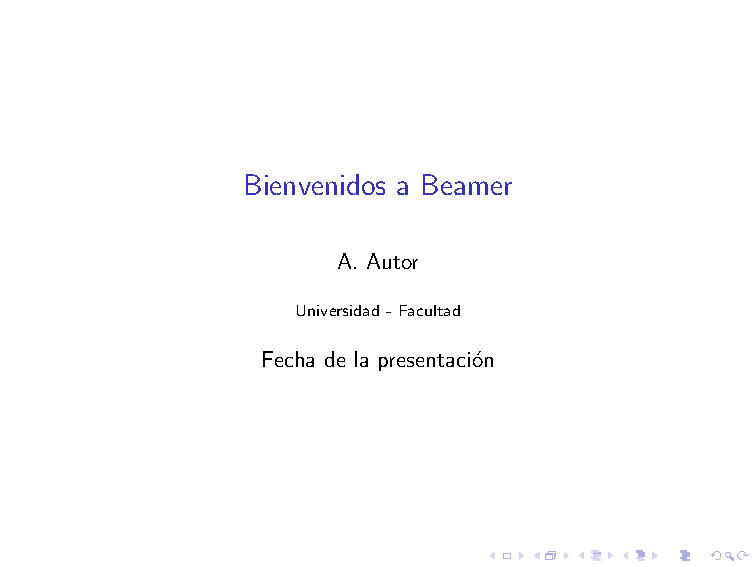
\includegraphics[width=\textwidth,clip,trim=1in 1in 1in 1in]{beamer-minimal.pdf}
  \end{minipage}
\end{frame}

%%%%%%%%%%%%%%%%%%%%%%%%%%%%%%%%%%%%%%%%%%%%%%%%%%%%%%%%%%%%%%%%%%%%%%%%%%%%%%%
%%%%%%%%%%%%%%%%%%%%%%%%%%%%%%%%%%%%%%%%%%%%%%%%%%%%%%%%%%%%%%%%%%%%%%%%%%%%%%%
%%%%%%%%%%%%%%%%%%%%%%%%%%%%%%%%%%%%%%%%%%%%%%%%%%%%%%%%%%%%%%%%%%%%%%%%%%%%%%%
\begin{frame}[fragile]{\insertsection: Sigamos con nuevos concetos}
  
  \begin{itemize}
  \item A medida que avancemos a través de las siguientes
    diapositivas pruebe los ejemplos escribiéndolos sobre la
    plataforma Overleaf.
  \end{itemize}
  \vskip 2ex
  \begin{center}
    \fbox{\href{\wlnewdoc{beamer-minimal.tex}}{%
        Click para abrir el documento de ejemplo en \wllogo{}}}
  \end{center}
\end{frame}

%%%%%%%%%%%%%%%%%%%%%%%%%%%%%%%%%%%%%%%%%%%%%%%%%%%%%%%%%%%%%%%%%%%%%%%%%%%%%%%
%%%%%%%%%%%%%%%%%%%%%%%%%%%%%%%%%%%%%%%%%%%%%%%%%%%%%%%%%%%%%%%%%%%%%%%%%%%%%%%
%%%%%%%%%%%%%%%%%%%%%%%%%%%%%%%%%%%%%%%%%%%%%%%%%%%%%%%%%%%%%%%%%%%%%%%%%%%%%%%
\begin{frame}[fragile]
  \frametitle{\insertsection: Diapositivas}
  \begin{itemize}
  \item Utilice \cmdbs{frametitle} para darle un título al cuadro.
  \item Luego agregue contenido a la diapositiva.
  \item El código para esta diapositiva se ve así
    \vskip 2ex
    \inputminted[fontsize=\scriptsize,frame=single,resetmargins]{latex}%
    {es/beamer-frame.tex}
  \end{itemize}
\end{frame}

%%%%%%%%%%%%%%%%%%%%%%%%%%%%%%%%%%%%%%%%%%%%%%%%%%%%%%%%%%%%%%%%%%%%%%%%%%%%%%% 
%%%%%%%%%%%%%%%%%%%%%%%%%%%%%%%%%%%%%%%%%%%%%%%%%%%%%%%%%%%%%%%%%%%%%%%%%%%%%%% 
%%%%%%%%%%%%%%%%%%%%%%%%%%%%%%%%%%%%%%%%%%%%%%%%%%%%%%%%%%%%%%%%%%%%%%%%%%%%%%% 
\begin{frame}[fragile]{\insertsection: Secciones}
  \begin{itemize}
  \item Puede agrupar sus diapositivas en secciones, y de
    esta forma  \bftt{beamer} las utilizará para crear un esquema automático.
  \item Para generar un esquema de su presentación, utilice el comando
    \cmdbs{tableofcontents}. Aquí esta uno para esta presentación. La
    opción \bftt{currentsection} resalta la actual sección.
    \vskip 2ex
    \begin{exampletwouptiny}
\tableofcontents[currentsection]
    \end{exampletwouptiny}
  \end{itemize}
\end{frame}

%%%%%%%%%%%%%%%%%%%%%%%%%%%%%%%%%%%%%%%%%%%%%%%%%%%%%%%%%%%%%%%%%%%%%%%%%%%%%%% 
%%%%%%%%%%%%%%%%%%%%%%%%%%%%%%%%%%%%%%%%%%%%%%%%%%%%%%%%%%%%%%%%%%%%%%%%%%%%%%%
%%%%%%%%%%%%%%%%%%%%%%%%%%%%%%%%%%%%%%%%%%%%%%%%%%%%%%%%%%%%%%%%%%%%%%%%%%%%%%%
\begin{frame}[fragile]{\insertsection: Múltiples Columnas}
  \begin{columns}
    \begin{column}{0.4\textwidth}
      \begin{itemize}
      \item Utilice los entornos  \bftt{columns} y \bftt{column} para
        dividir la diapositiva en columnas.
      \item El argumento para cada comando  \bftt{column} determina su
        ancho.
      \item Vea también el paquete \bftt{multicol}, que
        automáticamente divide su contenido en columnas.
      \end{itemize}
    \end{column}
    \begin{column}{0.6\textwidth}
      \begin{minted}[fontsize=\scriptsize,frame=single]{latex}
\begin{columns}
  \begin{column}{0.4\textwidth}
    \begin{itemize}
    \item Utilice los entornos  ...
    \item El argumento ...
    \item Vea tambi\'en el ...
    \end{itemize}
  \end{column}
  \begin{column}{0.6\textwidth}
    % segunda columna
  \end{column}
\end{columns}
      \end{minted}
    \end{column}
  \end{columns}
\end{frame}

%%%%%%%%%%%%%%%%%%%%%%%%%%%%%%%%%%%%%%%%%%%%%%%%%%%%%%%%%%%%%%%%%%%%%%%%%%%%%%%
%%%%%%%%%%%%%%%%%%%%%%%%%%%%%%%%%%%%%%%%%%%%%%%%%%%%%%%%%%%%%%%%%%%%%%%%%%%%%%%
%%%%%%%%%%%%%%%%%%%%%%%%%%%%%%%%%%%%%%%%%%%%%%%%%%%%%%%%%%%%%%%%%%%%%%%%%%%%%%%
\begin{frame}[fragile]{\insertsection: Resaltar texto}
  \begin{itemize}
    
  \item Utilice  \cmdbs{emph} o \cmdbs{alert} para resaltar texto:
    \vskip 1ex
    \begin{exampletwouptiny}
Debo \emph{enfatizar} que 
esto es un punto \alert{importante}.
    \end{exampletwouptiny}
    \vskip 1ex
    
  \item O especificar,
    \vskip 1ex
    \begin{exampletwouptiny}
Texto en \textbf{negrita}.
Texto en \textit{italica}.
    \end{exampletwouptiny}
    \vskip 1ex
    
  \item O especificar un color:
    \vskip 1ex
    \begin{exampletwouptiny}
Se \textcolor{red}{detiene}
e \textcolor{green}{inicia}.
    \end{exampletwouptiny}
    \vskip 1ex
  \item Vea \url{http://userpages.umbc.edu/~rostamia/beamer/quickstart-Z-H-25.html}
    para más colores y colores personalizados.
  \end{itemize}
\end{frame}

%%%%%%%%%%%%%%%%%%%%%%%%%%%%%%%%%%%%%%%%%%%%%%%%%%%%%%%%%%%%%%%%%%%%%%%%%%%%%%%
%%%%%%%%%%%%%%%%%%%%%%%%%%%%%%%%%%%%%%%%%%%%%%%%%%%%%%%%%%%%%%%%%%%%%%%%%%%%%%%
%%%%%%%%%%%%%%%%%%%%%%%%%%%%%%%%%%%%%%%%%%%%%%%%%%%%%%%%%%%%%%%%%%%%%%%%%%%%%%%
\begin{frame}[fragile]{\insertsection: Figuras}
  \begin{itemize}
  \item Utilice  \cmdbs{includegraphics} desde el paquete  \bftt{graphicx}.
  \item El entorno \bftt{figure} centra la imagen por defecto en \bftt{beamer}.
    \vskip 2ex
    \begin{exampletwouptiny}
\begin{figure}
  \includegraphics[
  width=0.5\textwidth]{es/big_chick}
\end{figure}
    \end{exampletwouptiny}
  \end{itemize}
\end{frame}

%%%%%%%%%%%%%%%%%%%%%%%%%%%%%%%%%%%%%%%%%%%%%%%%%%%%%%%%%%%%%%%%%%%%%%%%%%%%%%%
%%%%%%%%%%%%%%%%%%%%%%%%%%%%%%%%%%%%%%%%%%%%%%%%%%%%%%%%%%%%%%%%%%%%%%%%%%%%%%%
%%%%%%%%%%%%%%%%%%%%%%%%%%%%%%%%%%%%%%%%%%%%%%%%%%%%%%%%%%%%%%%%%%%%%%%%%%%%%%%
\begin{frame}[fragile]{\insertsection: Tablas}
  \begin{itemize}
  \item Las tablas en \LaTeX{} requieren un tiempo para acostumbrarse.
%  \item Utilice el entorno \bftt{tabular} desde el paquete
%\bftt{tabularx}.
  \item El argumento especifica la alineación de las columnas ---
\textbf{l}eft, \textbf{r}ight, \textbf{r}ight.
    \begin{exampletwouptiny}
\begin{tabular}{lrr}
  Art.   & Cant. & Uni. \$ \\
  DVD    & 1     & 19.99   \\
  Sonido & 2     & 39.99   \\
  Cable  & 3     & 1.99    \\
\end{tabular}
    \end{exampletwouptiny}
  \item También se especifican las líneas verticales; utilice el
comando \cmdbs{hline} para las líneas horizontales.
    \begin{exampletwouptiny}
\begin{tabular}{|l|r|r|}     \hline
  Art.   & Cant. & Uni. \$ \\\hline
  DVD    & 1     & 19.99   \\
  Sonido & 2     & 39.99   \\
  Cable  & 3     & 1.99    \\\hline
\end{tabular}
    \end{exampletwouptiny}
  \item Utilice un ampersand \keystrokebftt{\&} para separarlas
columnas y una doble barra invertida
\keystrokebftt{\bs}\keystrokebftt{\bs} para comenzar una nueva
fila.
  \end{itemize}
\end{frame}

%%%%%%%%%%%%%%%%%%%%%%%%%%%%%%%%%%%%%%%%%%%%%%%%%%%%%%%%%%%%%%%%%%%%%%%%%%%%%%% 
%%%%%%%%%%%%%%%%%%%%%%%%%%%%%%%%%%%%%%%%%%%%%%%%%%%%%%%%%%%%%%%%%%%%%%%%%%%%%%% 
%%%%%%%%%%%%%%%%%%%%%%%%%%%%%%%%%%%%%%%%%%%%%%%%%%%%%%%%%%%%%%%%%%%%%%%%%%%%%%% 
\begin{frame}[fragile]{\insertsection: Bloques}
  \begin{itemize}
  \item Un entorno  \bftt{block} realiza un cuadro titulado.

    \begin{exampletwouptiny}
\begin{block}{Dato interesante}
  Esto es importante.
\end{block}

\begin{alertblock}{Advertencia}
  Esto es muy importante!
\end{alertblock}
    \end{exampletwouptiny}
    
  \item Estos tipos de bloques dependen del tema utilizado\ldots
  \end{itemize}
\end{frame}

%%%%%%%%%%%%%%%%%%%%%%%%%%%%%%%%%%%%%%%%%%%%%%%%%%%%%%%%%%%%%%%%%%%%%%%%%%%%%%% 
%%%%%%%%%%%%%%%%%%%%%%%%%%%%%%%%%%%%%%%%%%%%%%%%%%%%%%%%%%%%%%%%%%%%%%%%%%%%%%% 
%%%%%%%%%%%%%%%%%%%%%%%%%%%%%%%%%%%%%%%%%%%%%%%%%%%%%%%%%%%%%%%%%%%%%%%%%%%%%%% 
\begin{frame}[fragile]
  \frametitle{\insertsection: Temas}
  \begin{itemize}
  \item Personalice el aspecto de su presentación utilizando temas.
  \item Vea \url{http://deic.uab.es/~iblanes/beamer_gallery/index_by_theme.html}
    para una gran colección de temas.
  \end{itemize}
  \begin{minipage}{0.55\linewidth}
    \inputminted[fontsize=\scriptsize,frame=single,resetmargins]{latex}%
    {es/beamer-theme.tex}
  \end{minipage}
  \begin{minipage}{0.35\linewidth}
    % trim: l b r t
    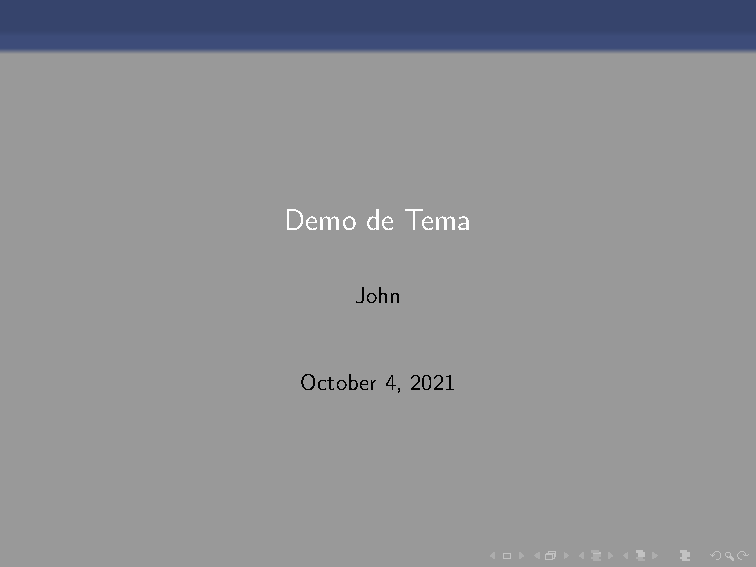
\includegraphics[width=\textwidth]{beamer-theme.pdf}
  \end{minipage}
\end{frame}

%%%%%%%%%%%%%%%%%%%%%%%%%%%%%%%%%%%%%%%%%%%%%%%%%%%%%%%%%%%%%%%%%%%%%%%%%%%%%%%
%%%%%%%%%%%%%%%%%%%%%%%%%%%%%%%%%%%%%%%%%%%%%%%%%%%%%%%%%%%%%%%%%%%%%%%%%%%%%%%
%%%%%%%%%%%%%%%%%%%%%%%%%%%%%%%%%%%%%%%%%%%%%%%%%%%%%%%%%%%%%%%%%%%%%%%%%%%%%%%
\begin{frame}[fragile]{\insertsection: Animación}
  \begin{itemize}
  \item Un cuadro puede generar múltiples diapositivas.
  \item Utilice el comando \cmdbs{pause} para mostrar sólo una parte
    de una diapositiva.
    \vskip 2ex
    \begin{exampletwouptinynoframe}
\begin{itemize}
\item Puede apreciar
  \pause \item la pausa?
\end{itemize}
    \end{exampletwouptinynoframe}
    \vskip 2ex
  \item Hay muchas maneras de hacer animaciones en \bftt{beamer}; vea
    también los comandos \cmdbs{only}, \cmdbs{alt}, y \cmdbs{uncover}.
  \end{itemize}
\end{frame}

%%%%%%%%%%%%%%%%%%%%%%%%%%%%%%%%%%%%%%%%%%%%%%%%%%%%%%%%%%%%%%%%%%%%%%%%%%%%%%%
%%%%%%%%%%%%%%%%%%%%%%%%%%%%%%%%%%%%%%%%%%%%%%%%%%%%%%%%%%%%%%%%%%%%%%%%%%%%%%%
%%%%%%%%%%%%%%%%%%%%%%%%%%%%%%%%%%%%%%%%%%%%%%%%%%%%%%%%%%%%%%%%%%%%%%%%%%%%%%%
\begin{frame}[fragile]{\insertsection: Ejercicio}

  Recrear la nota de  Peter Norvig ``Gettysburg Powerpoint Presentation'' en \bftt{beamer}.\footnote{\url{http://norvig.com/Gettysburg}}
  
  \begin{enumerate}
  \item Abra este ejercicio en  \wllogo{}:
    \begin{center}
      \fbox{\href{\wlnewdoc{beamer-exercise.tex}}{%
          Click para abrir el ejercicio en  \wllogo{}}}
    \end{center}
    \vskip 2ex
  \item Descargue esta imagen en su computadora y súbalo a  \wllogo{}
    a través del menú files.
    \begin{center}
      \fbox{\href{\fileuri/gettysburg_graph.png?dl=1}{Click para
          descargar imagen}}
    \end{center}
    \vskip 2ex
  \item Agregue comandos  \LaTeX{} al texto para logra una
    presentación similar a esta:
    \begin{center}
      \fbox{\href{\fileuri/beamer-exercise-solution.pdf}{%
          Click para abril el documento modelo}}
    \end{center}
  \end{enumerate}
\end{frame}

%%%%%%%%%%%%%%%%%%%%%%%%%%%%%%%%%%%%%%%%%%%%%%%%%%%%%%%%%%%%%%%%%%%%%%%%%%%%%%%
%%%%%%%%%%%%%%%%%%%%%%%%%%%%%%%%%%%%%%%%%%%%%%%%%%%%%%%%%%%%%%%%%%%%%%%%%%%%%%%
%%%%%%%%%%%%%%%%%%%%%%%%%%%%%%%%%%%%%%%%%%%%%%%%%%%%%%%%%%%%%%%%%%%%%%%%%%%%%%%
\section{Notas con \protect\bftt{todonotes}}

%%%%%%%%%%%%%%%%%%%%%%%%%%%%%%%%%%%%%%%%%%%%%%%%%%%%%%%%%%%%%%%%%%%%%%%%%%%%%%%
%%%%%%%%%%%%%%%%%%%%%%%%%%%%%%%%%%%%%%%%%%%%%%%%%%%%%%%%%%%%%%%%%%%%%%%%%%%%%%%
%%%%%%%%%%%%%%%%%%%%%%%%%%%%%%%%%%%%%%%%%%%%%%%%%%%%%%%%%%%%%%%%%%%%%%%%%%%%%%%
\begin{frame}[fragile]{\insertsection}
  \begin{itemize}
  \item El comando  \cmdbs{todo} del paquete  \bftt{todonotes}  es
    ideal cuando se quiere dejar notas para uno mismo y sus
    colaboradores, quienes están redactando un documento.
    \begin{exampletwouptiny}
\todo{agregar resultados}
\todo[color=blue!20]{soluci\'on}
    \end{exampletwouptiny}
    \vskip 2ex
  \item Consejos: defina sus propios comandos con \cmdbs{newcommand}
    \begin{minted}[fontsize=\scriptsize,frame=single]{latex}
\newcommand{\alicia}[1]{\todo[color=green!40]{#1}}
\newcommand{\juan}[1]{\todo[color=purple!40]{#1}}
    \end{minted}
    Esto puede ahorrar un montón de escritura:
    \begin{exampletwouptiny}
\alicia{agregar resultados}
\juan{soluci\'on}
    \end{exampletwouptiny}
  \end{itemize}
\end{frame}

%%%%%%%%%%%%%%%%%%%%%%%%%%%%%%%%%%%%%%%%%%%%%%%%%%%%%%%%%%%%%%%%%%%%%%%%%%%%%%%
%%%%%%%%%%%%%%%%%%%%%%%%%%%%%%%%%%%%%%%%%%%%%%%%%%%%%%%%%%%%%%%%%%%%%%%%%%%%%%%
%%%%%%%%%%%%%%%%%%%%%%%%%%%%%%%%%%%%%%%%%%%%%%%%%%%%%%%%%%%%%%%%%%%%%%%%%%%%%%%
\begin{frame}[fragile]{\insertsection}
  \begin{columns}
    \begin{column}{0.4\textwidth}
      \begin{itemize}
      \item Sólo las notas en líneas son soportadas por beamer, pero las
        notas al margen están soportadas para la mayoría de
        las clases de documentos en \LaTeX{}.
      \item También hay práctico comando  \cmdbs{listoftodos}.
      \end{itemize}
    \end{column}
    \begin{column}{0.6\textwidth}
      \includegraphics[width=\textwidth,page=1]{es/todonotes-example}
    \end{column}
  \end{columns}
\end{frame}

\end{document}
